\graphicspath{{LiteratureReview/LiteratureReviewFigures/}}

\chapter{Literature Review}
\label{chap:Literature Review}
This chapter provides a better understanding of the background and information for the fulfilment of this research’s aims and objectives. First, a background of underground mining, the surveying of underground mines and the significance thereof is provided. Next, an overview is provided on the introduction of robotics in underground mining environments, including typical applications, current limitations, and state-of-the-art robotic platforms and multi-agent systems. Thirdly, the use of UAVs in underground mining is discussed, covering various UAV configurations, the basics of UAV construction, sensors used on UAVs in underground environments, and the offloading of computational tasks onto an on-board computer. 

Furthermore, a background on various Simultaneous Localisation and Mapping (SLAM) algorithms and sensor combinations is provided, followed by a section on SLAM performance measures and comparisons. Finally, a brief discussion on autonomous exploration, path planning and collision avoidance is provided, explaining their functionality and highlighting some state-of-the-art implementations.

%Section 1
\section{Underground Mine Surveying}
Underground mine surveying is a division of mining that is responsible for the measuring, calculating and mapping of information throughout the lifespan of a mine. Underground mine surveyors are therefore responsible for measuring existing and planned mine works to aid in the mines design, operational planning, and to determine and improve the safety of any mining operation~\cite{LabourSafety, Peter2023}. 

\subsection{Underground Mining}
During underground mining, minerals and ore material from beneath the Earth’s surface are extracted through techniques such as drilling, blasting, and mechanical excavation.  These processes are followed by the removal of the extracted ore and the installation of support structures to reinforce and stabilize the walls of the excavated areas. Common underground mining methods include room and pillar mining, used for flat lying ore bodies, in which the ore is excavated using a grid like approach, with pillars of ore left standing to support the overhead rock mass as seen in Figure~\ref{fig:MiningProcessesNum} (a). Sublevel open stoping is another common mining method, used for large ore bodies with a steep dip and regular shape, where primary vertical stopes are excavated first, while secondary stopes are left as support pillars, as depicted in Figure~\ref{fig:MiningProcessesNum} (b). Later the primary stopes are then backfilled and the secondary stopes are mined. A third common underground mining method is cut and fill mining, shown in Figure~\ref{fig:MiningProcessesNum} (c), this method is used for steep dip ore bodies with irregular shapes, in which the ore body is mined in horizontal slices using a repeated sequence of mining and backfilling layers, starting from the bottom most slice~\cite{Brady1985}.

\begin{figure}[!h]
    \centering
%     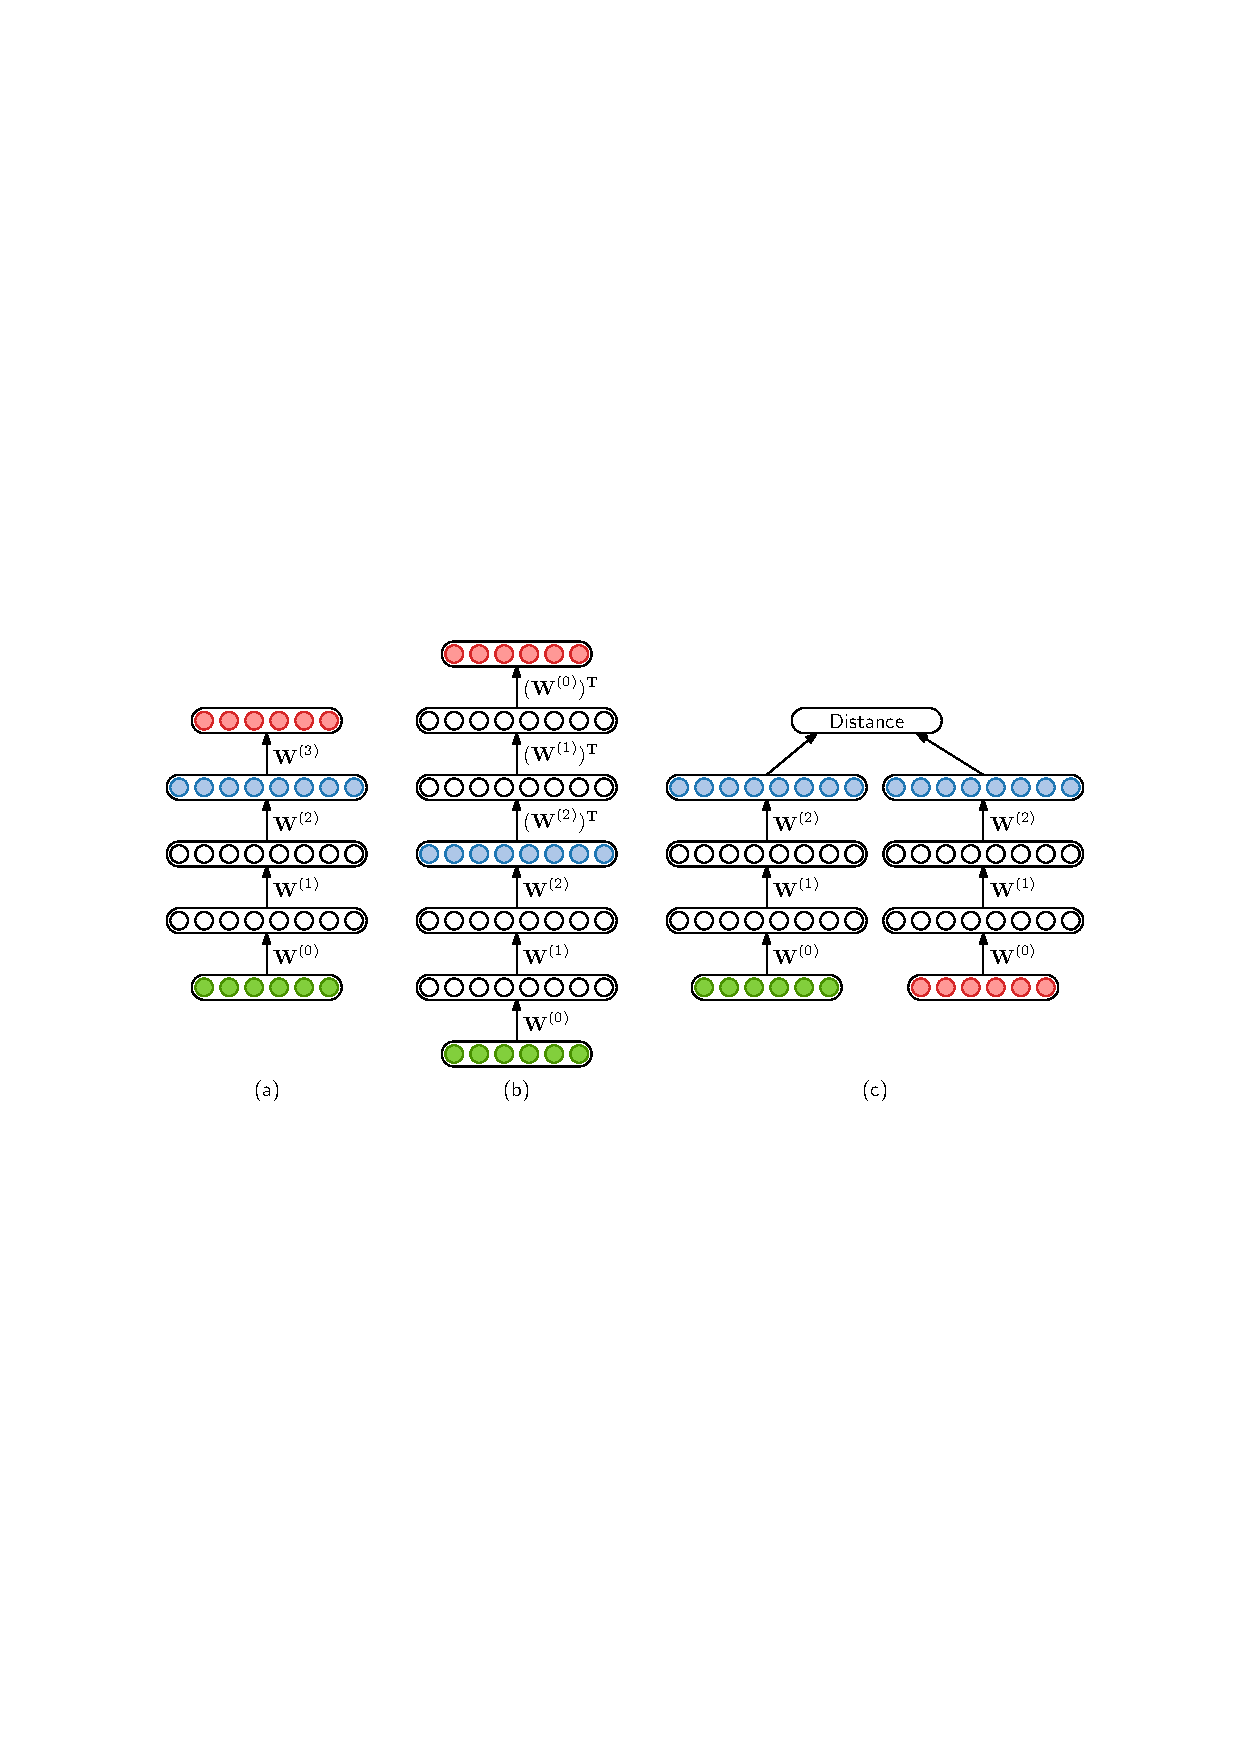
\includegraphics[width=\linewidth]{cae_siamese}
    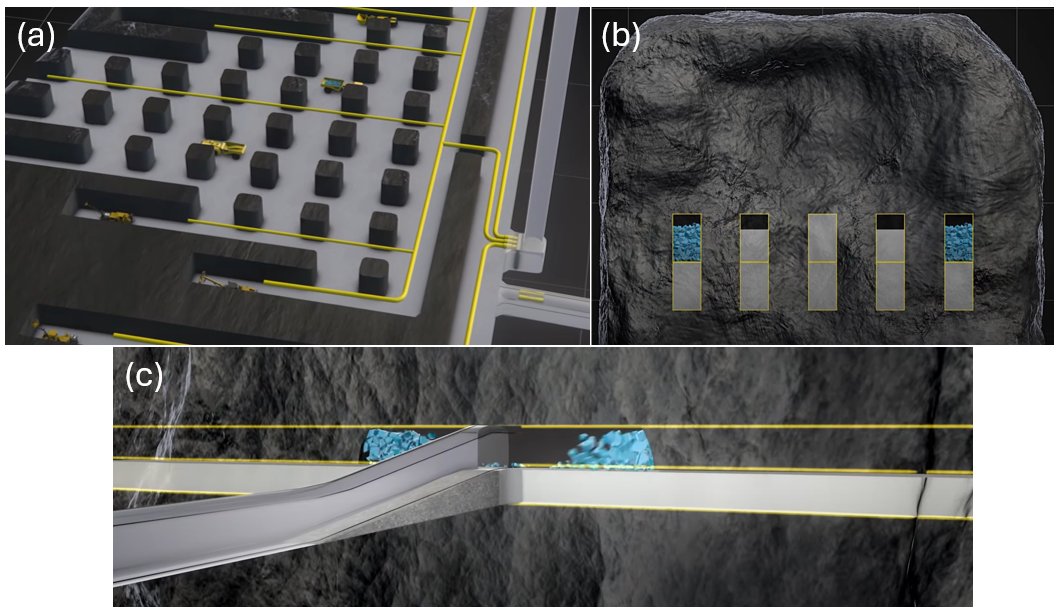
\includegraphics[width=0.918\linewidth]{MiningProcessesNum}
    \caption[Visualization of Different Underground Mining Processes]{
    Screen Captures of videos that visualize the methods of (a) room and pillar mining, (b) sublevel open stoping, and (c) cut and fill mining~\cite{Epiroc2019a, Epiroc2019b, Epiroc2019c}.
    }
    \label{fig:MiningProcessesNum}
\end{figure}

Throughout the underground mining  process, blasting is a critical step for breaking up hard rock. During this process holes are drilled into a rock face, filled with explosives and detonated in a controlled sequence to reduce ground vibrations as this can lead to structural damage, rock bursts and collapses~\cite{Xu2019}. After the blasting Process is complete, the fragmented ore pieces are then transported to the surface and support structures are put into place to further prevent collapses. These include Rock bolting, which composes of steel rods being anchored into rock strata to secure unstable layers~\cite{Wang2016}, shotcrete, which is sprayed concrete to reinforce tunnel walls~\cite{Brady1985}, and reinforced concrete pillars, supporting the overhead rock mass to prevent tunnel collapses~\cite{Cao2021}.

\subsection{Importance of Underground Mine Surveying}
Underground mine surveying is crucial for ensuring the precision and safety of the complex processes in underground mining operations described above. Specifically, mine surveying can be beneficial in mining aspects including efficient resource management, structural integrity monitoring and worker safety.

Firstly, underground mine surveying, specifically mapping of these environments, can aid in planning and post-extraction assessments, yielding critical information like the orientation of the stope face, tunnels and shafts as well as 3d detailed maps for drilling and blasting planning. Additionally, the Digital Terrain Models (DTMs) and 3D maps created by surveyors can be used for calculating excavated volumes, locations and sizes of underground support pillars, determining the accuracy of previous blasting operation and keeping track of any geological drifts~\cite{Ellmann2021}.

Furthermore, underground mine surveying plays a vital role in ensuring safety during mining operations and preventing serious accidents. Workplace safety is especially important in mining, as underground mines pose greater risks, including large-scale environmental damage and loss of human life, compared to many other work environments~\cite{John2021}. In contrast to open-pit mining, underground mining also poses greater risks due to ventilation issues and potential collapses. Common safety concerns in underground mining include rockfalls, support pillar collapses, water inflow, and gas leaks~\cite{Han2021}.  

Underground mine surveying can proactively help in mitigating these risks by identifying and managing potential hazards. Accurate surveying techniques provide detailed mapping and monitoring of post-mining deformations and can also help in the identification of structural integrity hazards, like collapsing pillars. An example of a potentially collapsing pillar undergoing spalling, the flaking off of material from support pillars, can be seen in Figure~\ref{fig:PillarCollapse1}, depicting the the progression of spalling in a gypsum mine pillar from 1996 to 2000\cite{Sorgi2011}.  Accurately assessing this kind of information can help predict structural instabilities, mitigating the risk of potential roof collapses and enhancing the safety of the mining personnel, specifically in room and pillar mining environments \cite{Yao2024}. 

\begin{figure}[!h]
    \centering
%     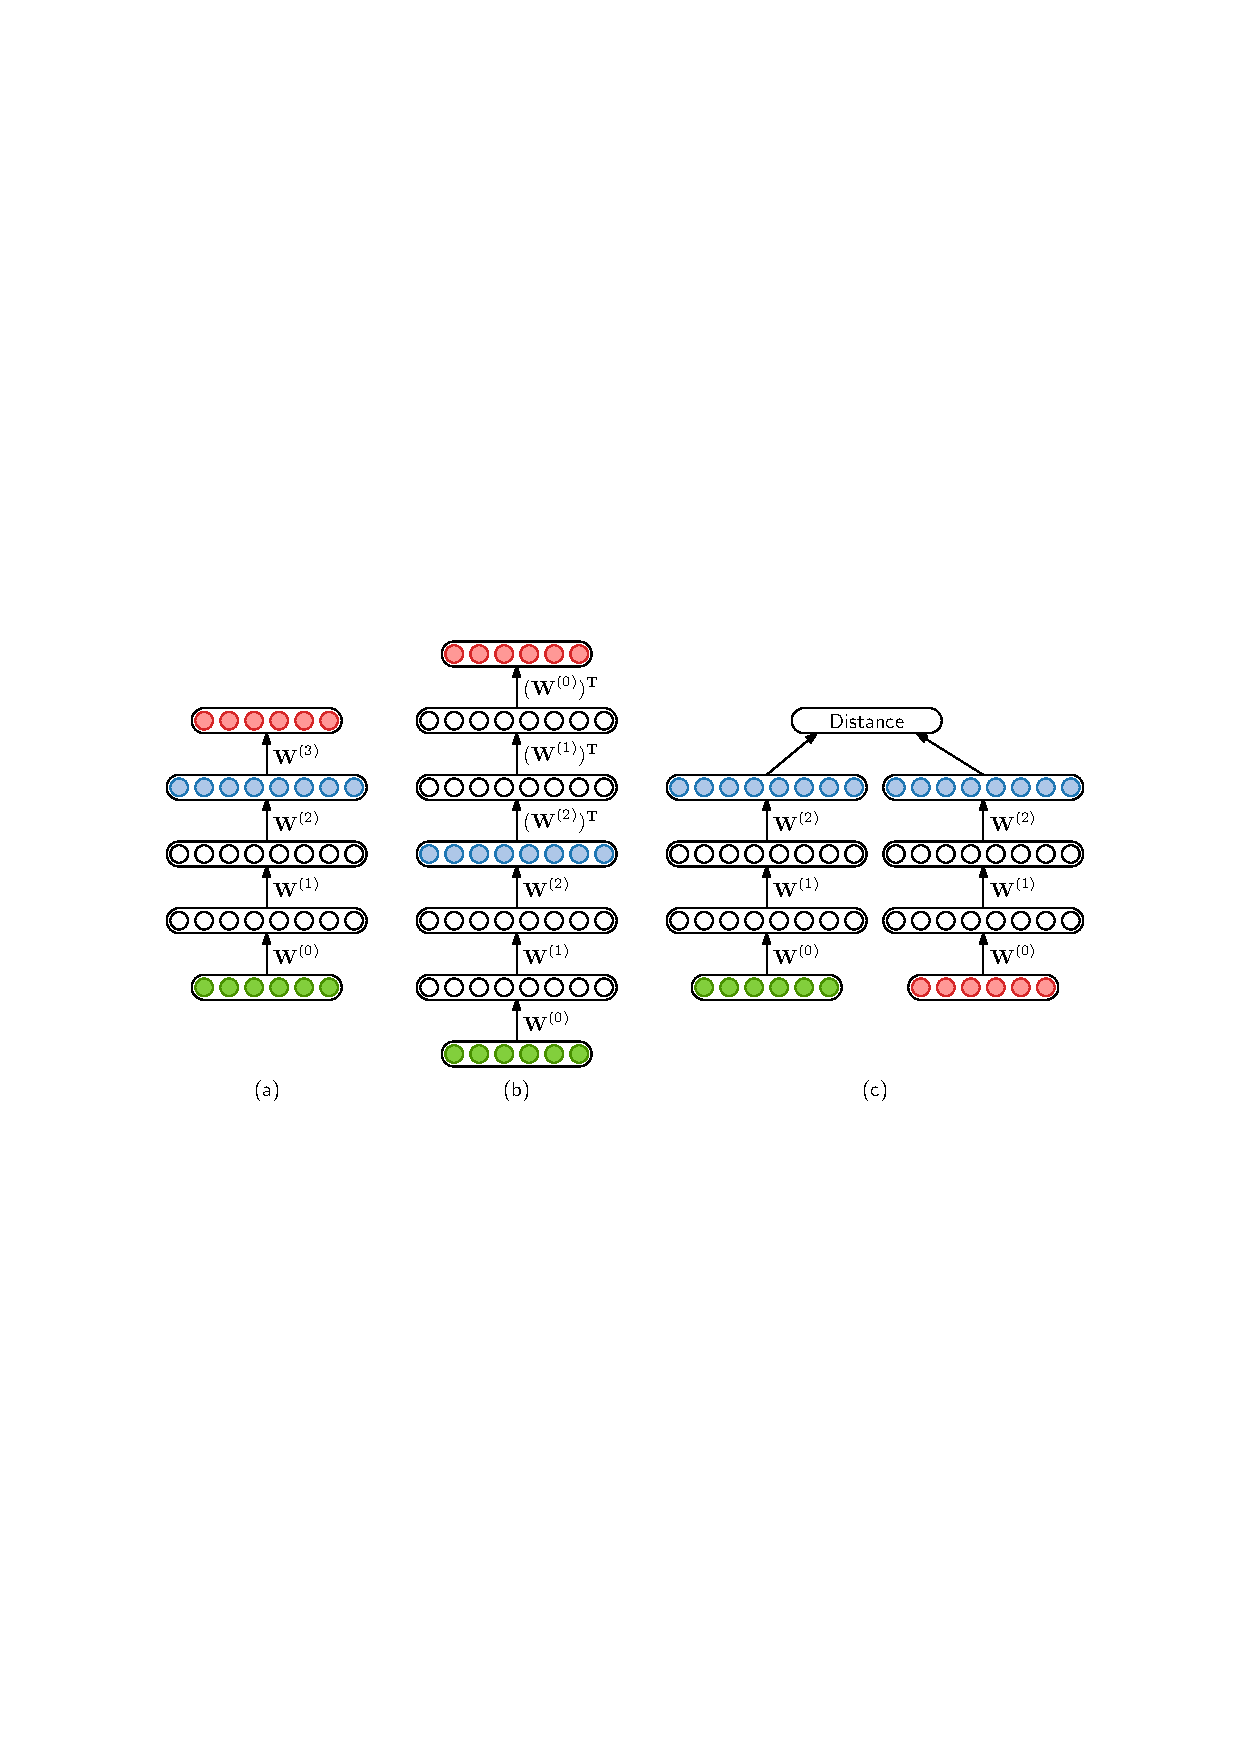
\includegraphics[width=\linewidth]{cae_siamese}
    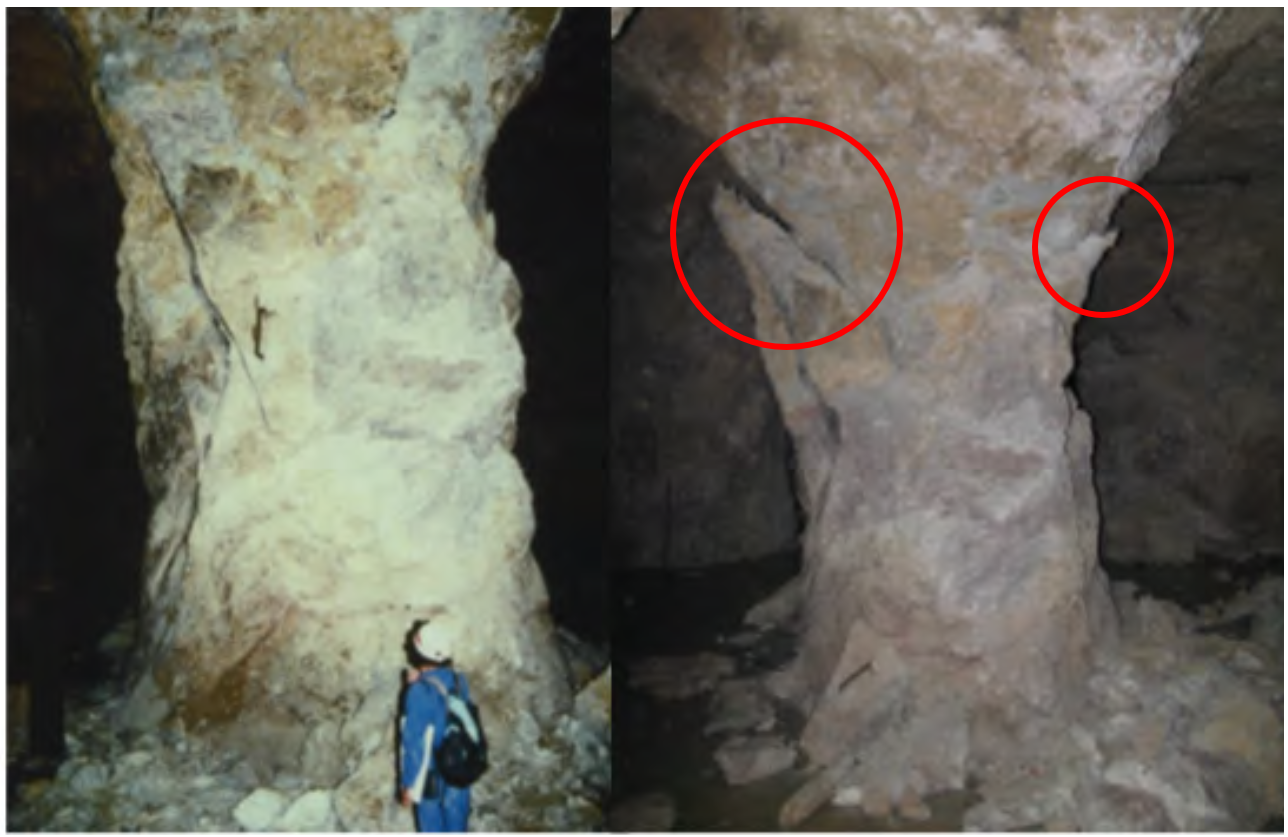
\includegraphics[width=0.75\linewidth]{PillarCollapse1}
    \caption[Example of a modern total station]{
    Example of a potentially collapsing pillar undergoing spalling in a gypsum mine pillar from 1996 to 2000\cite{Sorgi2011}.
    }
    \label{fig:PillarCollapse1}
\end{figure}



Moreover, underground mine surveying can facilitate the early detection of geological threats such as fault water leakage and groundwater seepage. This early detection allows for the timely implementation of waterproofing measures, reducing the potential risk of water related mining accidents \cite{Liu2019}. 

Furthermore, the integration of environmental monitoring sensors, help to continuously monitor the underground mining atmosphere for dangerous levels of hazardous gases. Some hazardous gases that can be found in underground mines include Carbon Dioxide (CO2), Carbon Monoxide(CO), Noxious gases (NO2, NO3, NO4), and flammable gases (CH4). The detection of abnormal levels of these hazardous gases can prevent incidents caused by exposure to toxic or explosive gases \cite{Anas2017}. 

Advanced surveying and monitoring methods therefore significantly contribute to safer working conditions in underground mining by allowing the proactive identification, assessment, and remediation of potential risks in these environments.

\subsection{Traditional Practices for Underground Mine Surveying}
The role of mining surveyors became a widespread and recognized profession in the 18th century. The primary instrument used during that time was the dial, a compass specifically designed for underground use, which can be seen in Figure~\ref{fig:SurveyHistory} (a). It was employed alongside measuring chains to map out the layout of underground environments. However, a significant drawback of this method was that iron tools and underground iron ore deposits would interfere with the dial's needle, leading to inaccuracies\cite{vanWegen2018}. 

In the 19th century, more advanced devices, such as the theodolite seen in Figure~\ref{fig:SurveyHistory} (b), were developed. These instruments consist of a telescope equipped with spirit levels and vertical quadrants to measure angles. By using theodolites alongside distance-measuring instruments, the traversing method was used to achieve significantly more accurate surveying results. During traversing, each survey station is used to observe and define the path to the next survey station or measured point, forming a surveying network. When this network is closed, meaning that the final point connects back to the starting point, the accuracy of the system could be determined\cite{vanWegen2018, Deakin2012}. 

In modern mining surveys, state-of-the-art total stations are used. These devices combine an electronic theodolite with an electronic distance sensor and are often equipped with electronic data storage, laser sighting, and GNSS modules to deliver very high levels of accuracy\cite{vanWegen2018}. A picture of a modern total station can be seen in Figure~\ref{fig:SurveyHistory} (c) below.

\begin{figure}[!h]
    \centering
%     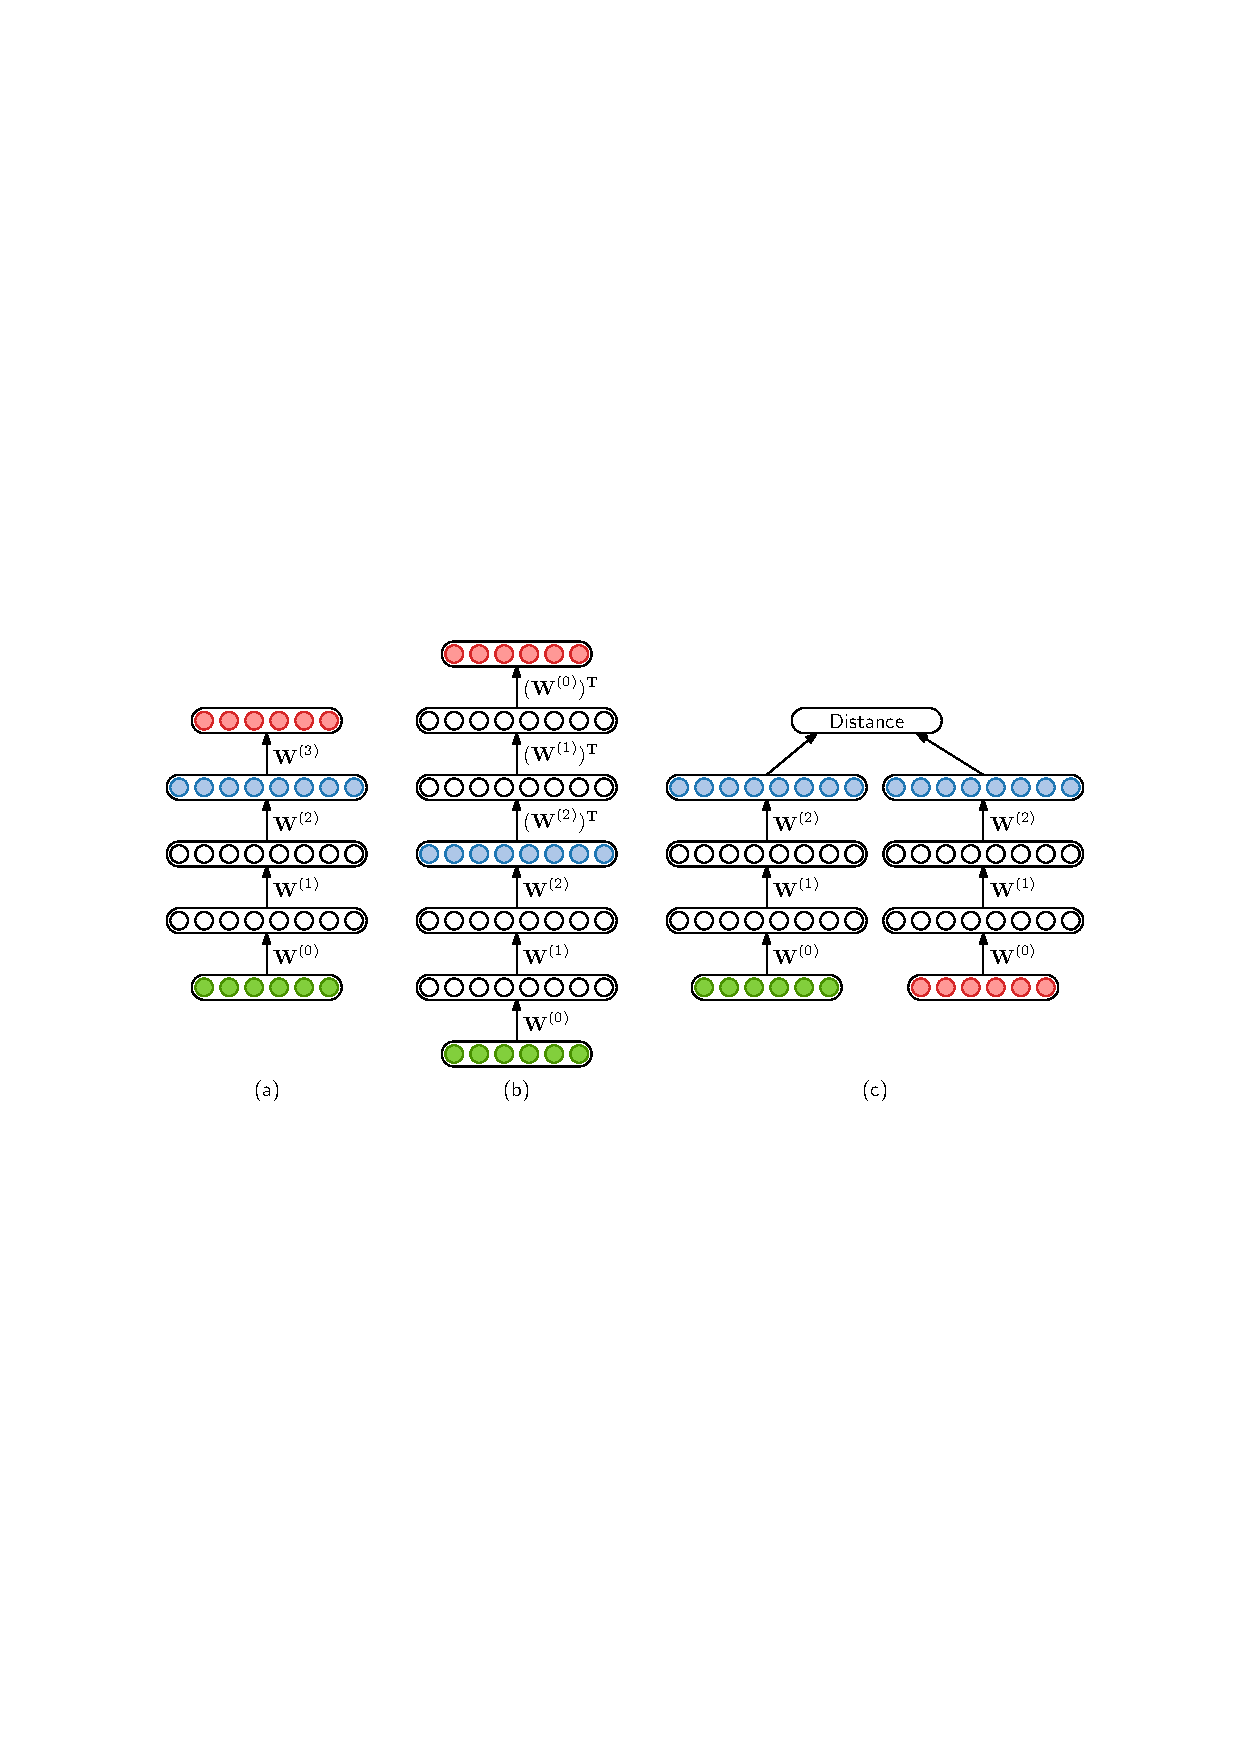
\includegraphics[width=\linewidth]{cae_siamese}
    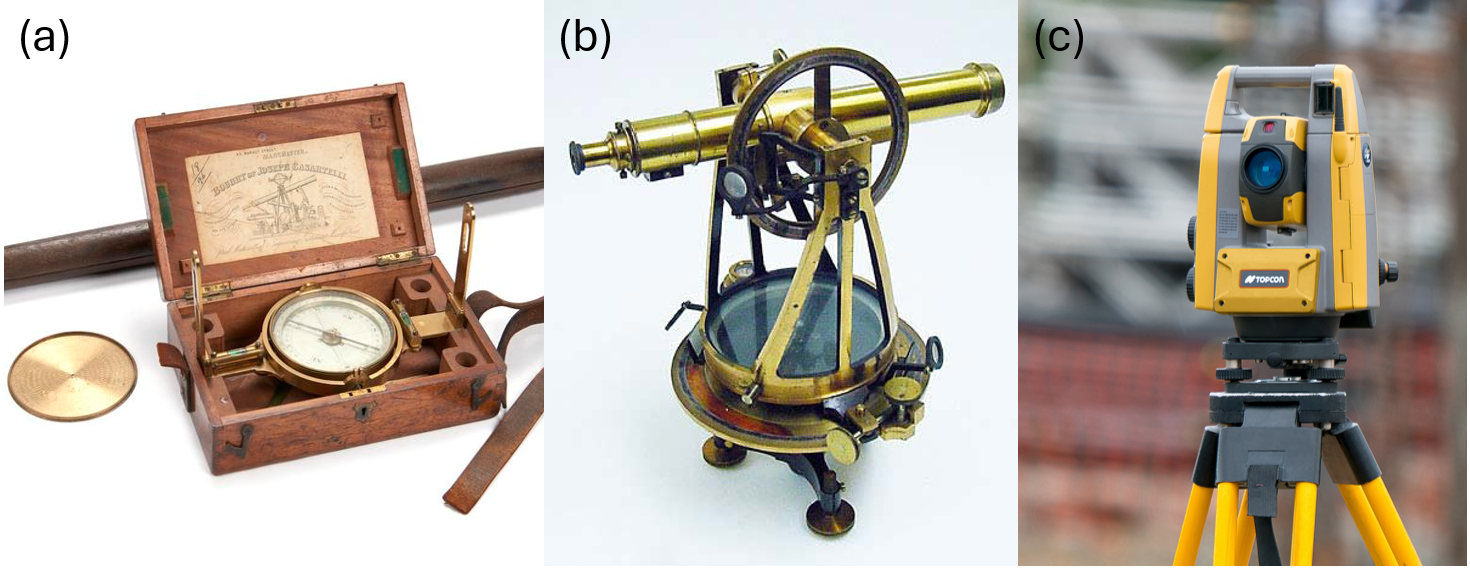
\includegraphics[width=0.918\linewidth]{SurveyHistory}
    \caption[Example of a modern total station]{
    Evolution of surveying instruments with (a) a mining dial, (b) a theodolite, and (c) a total station\cite{MinersDial, Topcon2020, NOAA2024}.
    Example of a modern total station\cite{Topcon2020}.
    }
    \label{fig:SurveyHistory}
\end{figure}


In underground mines, however, GNSS signals are ineffective, and traditional total stations must be used with classical methods such as traversing, triangulation or polar surveying. Additionally, it can become difficult to determine the accuracy of these devices in underground mines, if the tunnels don’t connect and no network closure can be established\cite{Laguillo2022, Buzatu2020}.

The traditional survey methods mentioned above, which use a point-wise survey station approach, are relatively simple but tend to be very time-consuming. Inaccuracies from omission errors can also be introduced due to uneven surfaces between subsequent surveying points\cite{Sobak2015}.

Over the last decade, advancements in surveying technology have led to the development of more modern methods capable of delivering fast, high-resolution data. Among these, laser scanning and photogrammetry are some of the methods at the forefront of innovation. They can be very effective for reconstructing complex geometries and environments by generating 3D point clouds. Compared to traditional surveying techniques, laser scanning and photogrammetry not only capture a greater volume of data in less time but also produce more detailed maps, including surface textures, uneven surfaces, and precise dimensions. Additionally, the processes are contactless with no danger of harming or manipulating any of the surveyed surfaces. Furthermore, techniques like terrestrial laser scanning (TLS) and photogrammetry data capture can be automated, reducing human interaction with the environment, enhancing human safety and further improving measurement precision. Because of these advantages, the most recent approaches have introduced robotics into underground mines to assist with data collection for surveying. Beyond strictly gathering survey data, the introduction of robotics in mining has also enabled various other applications within the underground mining environment\cite{Ellmann2021}. 



%Section 2
\section{Robotics in Mining}

\subsection{Different Applications for Robotics in Mining}
Surveying, Mapping, Inspection, Blasting......

% Laser scanning in underground mines:
% https://www.e3s-conferences.org/articles/e3sconf/pdf/2024/56/e3sconf_sep2024_01012.pdf 

\subsection{Challenging Conditions in Underground Mine Environments}

\subsection{GNSS Denied Environments and Sensors Used in Underground Mines}

\subsection{Current State of the Art Platforms/Implementations}

\subsection{Multi robot Systems}


%Section 3
\section{UAVs in Mining}

\subsection{UAV Configurations}

\subsection{Basic UAV Construction}

\subsubsection{Terminology and General Construction Considerations for Quadcopters}
1. roll, pitch, yaw\\
2. COG
\subsubsection{Basic Quadcopter Components}

\subsubsection{Flight Control Software/Autopilot}

\subsubsection{Integration of PX4 with ROS2 Humble and uXRCE-DDS}

\subsection{PX4 EKF2}

\subsection{Sensors Used on GNSS Denied UAVs}

\subsection{On Board Computing Module}
bla


%Section 4
\section{On Board SLAM}

\subsection{SLAM Overview}

\subsection{SLAM using Different Sensors}

\subsection{State of the Art SLAM Algorithms}

\subsubsection{RTABMAP}

\subsubsection{ORB-SLAM3}

\subsubsection{VDB Mapping}

\subsubsection{SpectacularAI Mapping}



\subsection{SLAM performance comparison parameters on computational limited devices}

%Section 5
\section{Autonomous navigation, path planning and collision avoidance}

\subsection{Autonomous navigation overview}

\subsection{State of the Art Autonomous Exploration Algorithms}

\subsubsection{FUEL}

\subsubsection{ERRT}

\subsubsection{UAV Frontier Exploration 3D}

\subsubsection{TARE Planner}

\subsubsection{FAR Planner}

\subsection{Path Planning and Obstacle Avoidance}

\subsubsection{Global Planner}

\subsubsection{Local Planner}